\section{Simulation Analysis}
\label{sec:simulation}

\subsection{Operating Point Analysis}

Table~\ref{tab:op} shows the simulated operating point results for the circuit
under analysis. Compared to the theoretical analysis results, one notices the
following differences: describe and explain the differences.

\begin{table}[h]
  \centering
  \begin{tabular}{|l|r|}
    \hline    
    {\bf Name} & {\bf Value [A or V]} \\ \hline
    @vx[i] & 9.804367e-04\\ \hline
@hc[i] & 3.412015e-05\\ \hline
@va[i] & -2.44092e-04\\ \hline
@gb[i] & -2.55448e-04\\ \hline
@id[current] & 1.014557e-03\\ \hline
@r1[i] & -2.44092e-04\\ \hline
@r2[i] & -2.55448e-04\\ \hline
@r3[i] & -1.13559e-05\\ \hline
@r4[i] & -1.22453e-03\\ \hline
@r5[i] & -1.27000e-03\\ \hline
@r6[i] & 9.804367e-04\\ \hline
@r7[i] & 9.804367e-04\\ \hline
n1 & 2.524677e-01\\ \hline
n2 & -5.18183e-01\\ \hline
n3 & 3.572797e-02\\ \hline
n4 & -4.90449e+00\\ \hline
n5 & 4.000301e+00\\ \hline
n6 & -6.93514e+00\\ \hline
n7 & -7.93124e+00\\ \hline
n8 & -6.93514e+00\\ \hline

  \end{tabular}
  \caption{Operating point. A variable preceded by @ is of type {\em current}
    and expressed in Ampere; other variables are of type {\it voltage} and expressed in
    Volt.}
  \label{tab:op}
\end{table}

\lipsum[1-1]


\subsection{Transient Analysis}

Figure~\ref{fig:trans} shows the simulated transient analysis results for the
circuit under analysis. Compared to the theoretical analysis results, one
notices the following differences: describe and explain the differences.

\begin{figure}[h] \centering
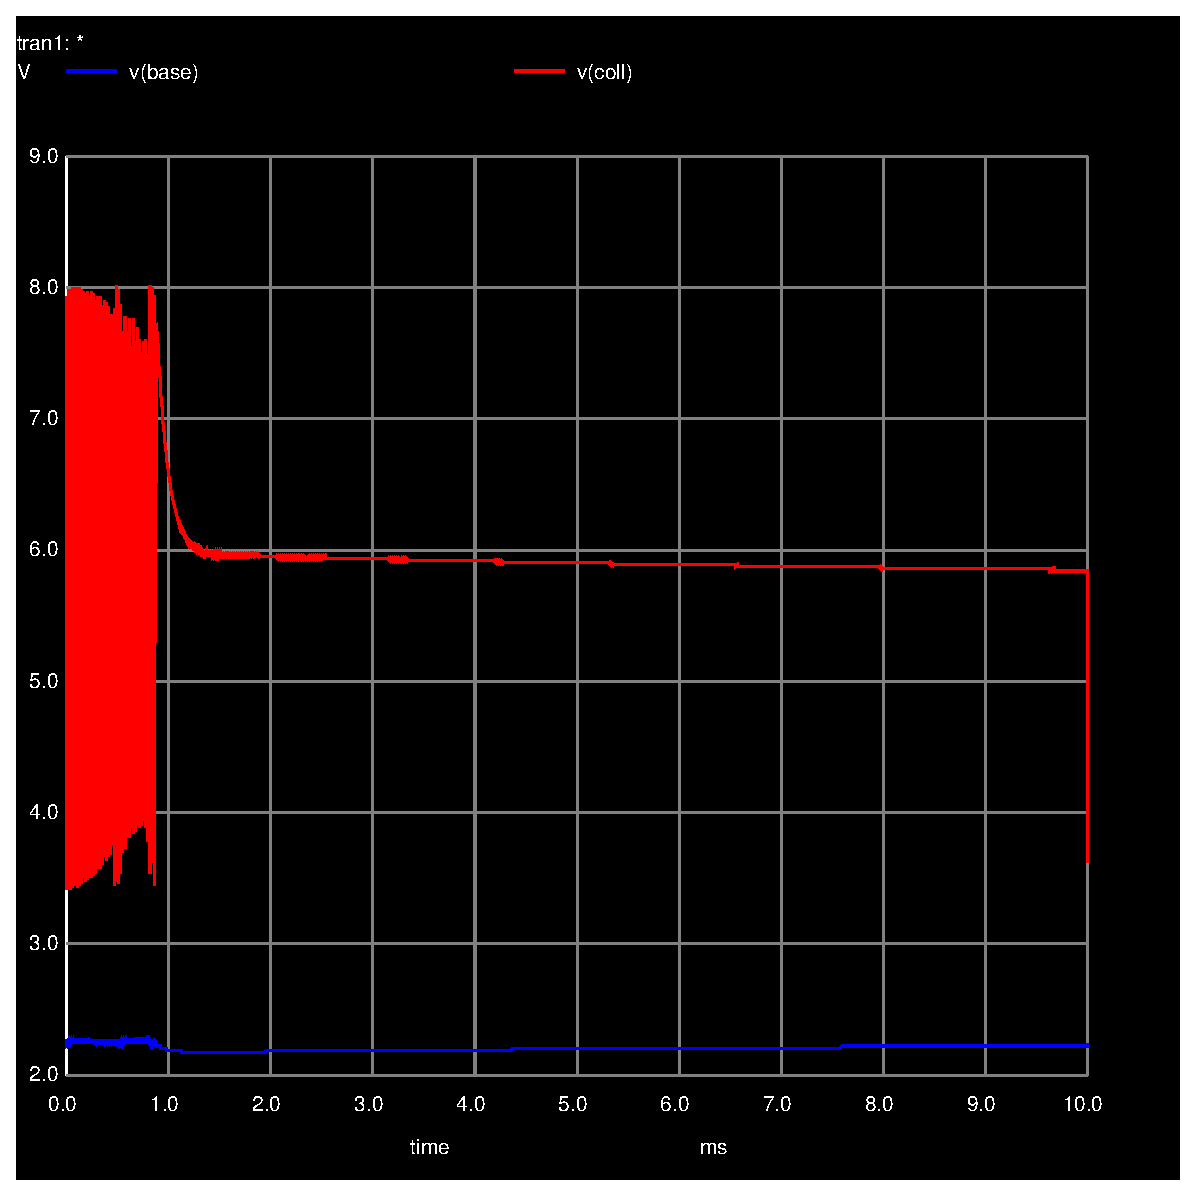
\includegraphics[width=0.6\linewidth]{trans.eps}
\caption{Transient output voltage}
\label{fig:trans}
\end{figure}

\lipsum[1-1]



\subsection{Frequency Analysis}

\subsubsection{Magnitude Response}

Figure~\ref{fig:acm} shows the magnitude of the frequency response for the
circuit under analysis. Compared to the theoretical analysis results, one
notices the following differences: describe and explain the differences.

\begin{figure}[h] \centering
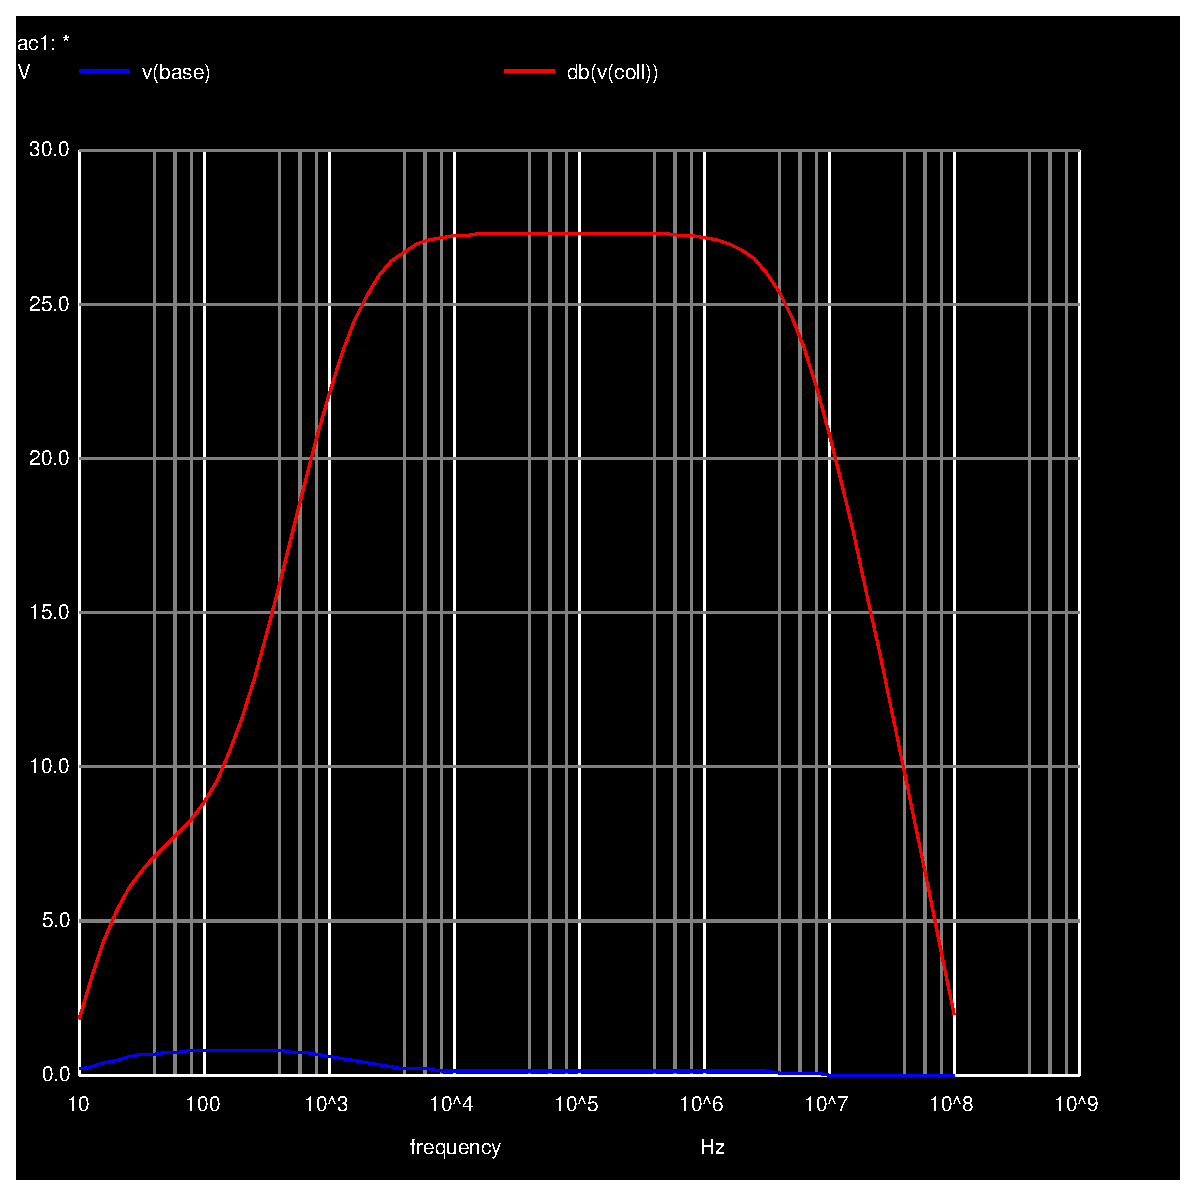
\includegraphics[width=0.6\linewidth]{acm.eps}
\caption{Magnitude response}
\label{fig:acm}
\end{figure}

\lipsum[1-1]

\subsubsection{Phase Response}

Figure~\ref{fig:acp} shows the magnitude of the frequency response for the
circuit under analysis. Compared to the theoretical analysis results, one
notices the following differences: describe and explain the differences.

\begin{figure}[h] \centering
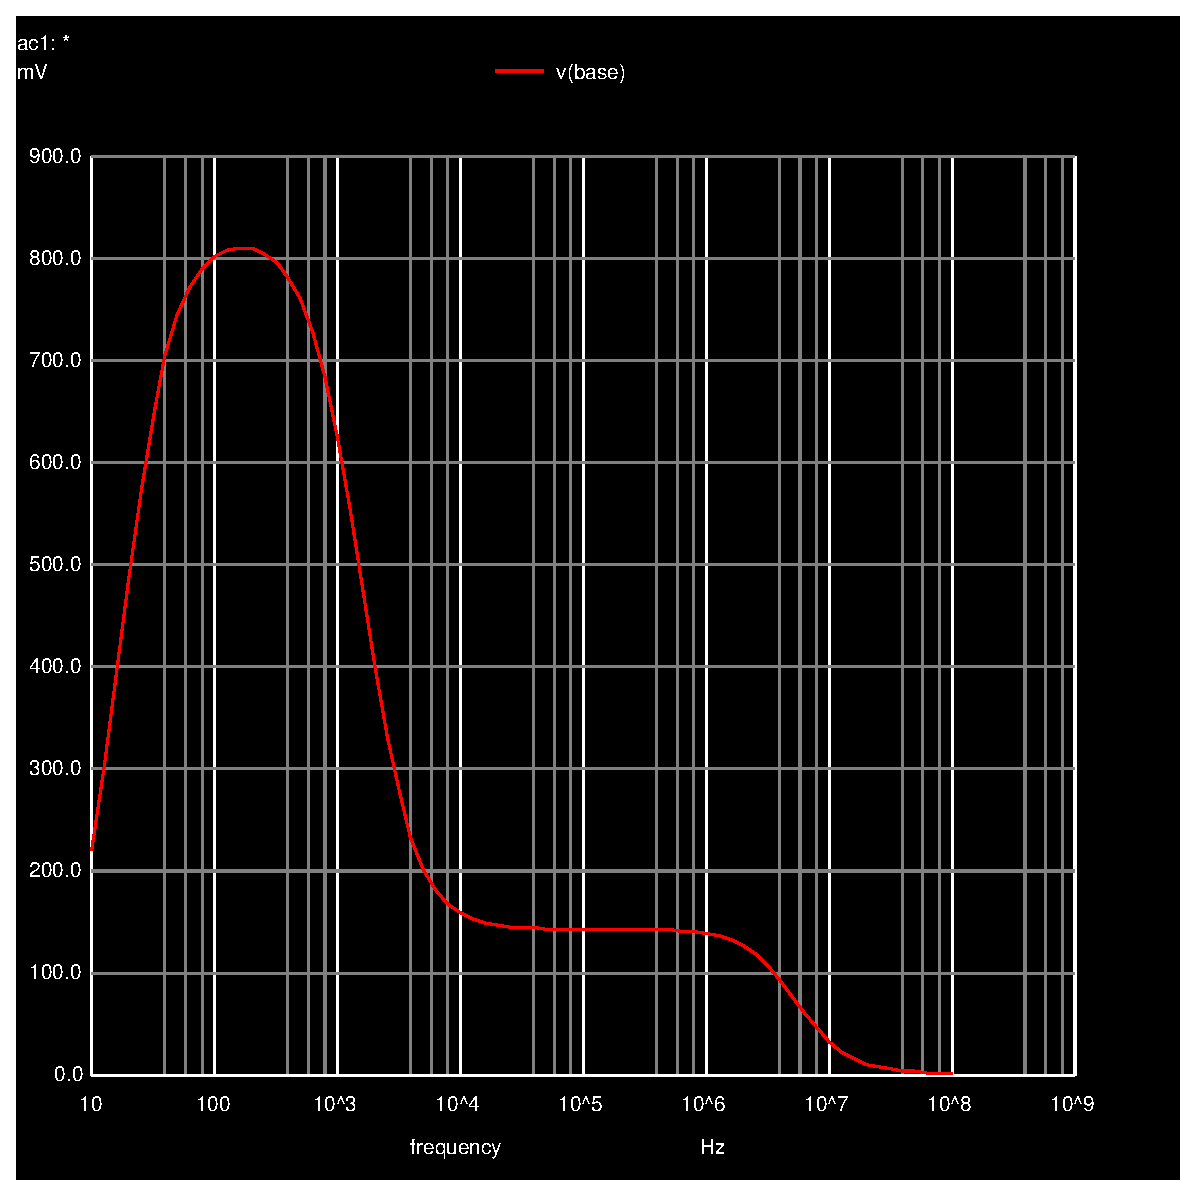
\includegraphics[width=0.6\linewidth]{acp.eps}
\caption{Phase response}
\label{fig:acp}
\end{figure}

\lipsum[1-1]

\subsubsection{Input Impedance}

Figure~\ref{fig:zim} shows the magnitude of the frequency response for the
circuit under analysis. Compared to the theoretical analysis results, one
notices the following differences: describe and explain the differences.

\begin{figure}[h] \centering
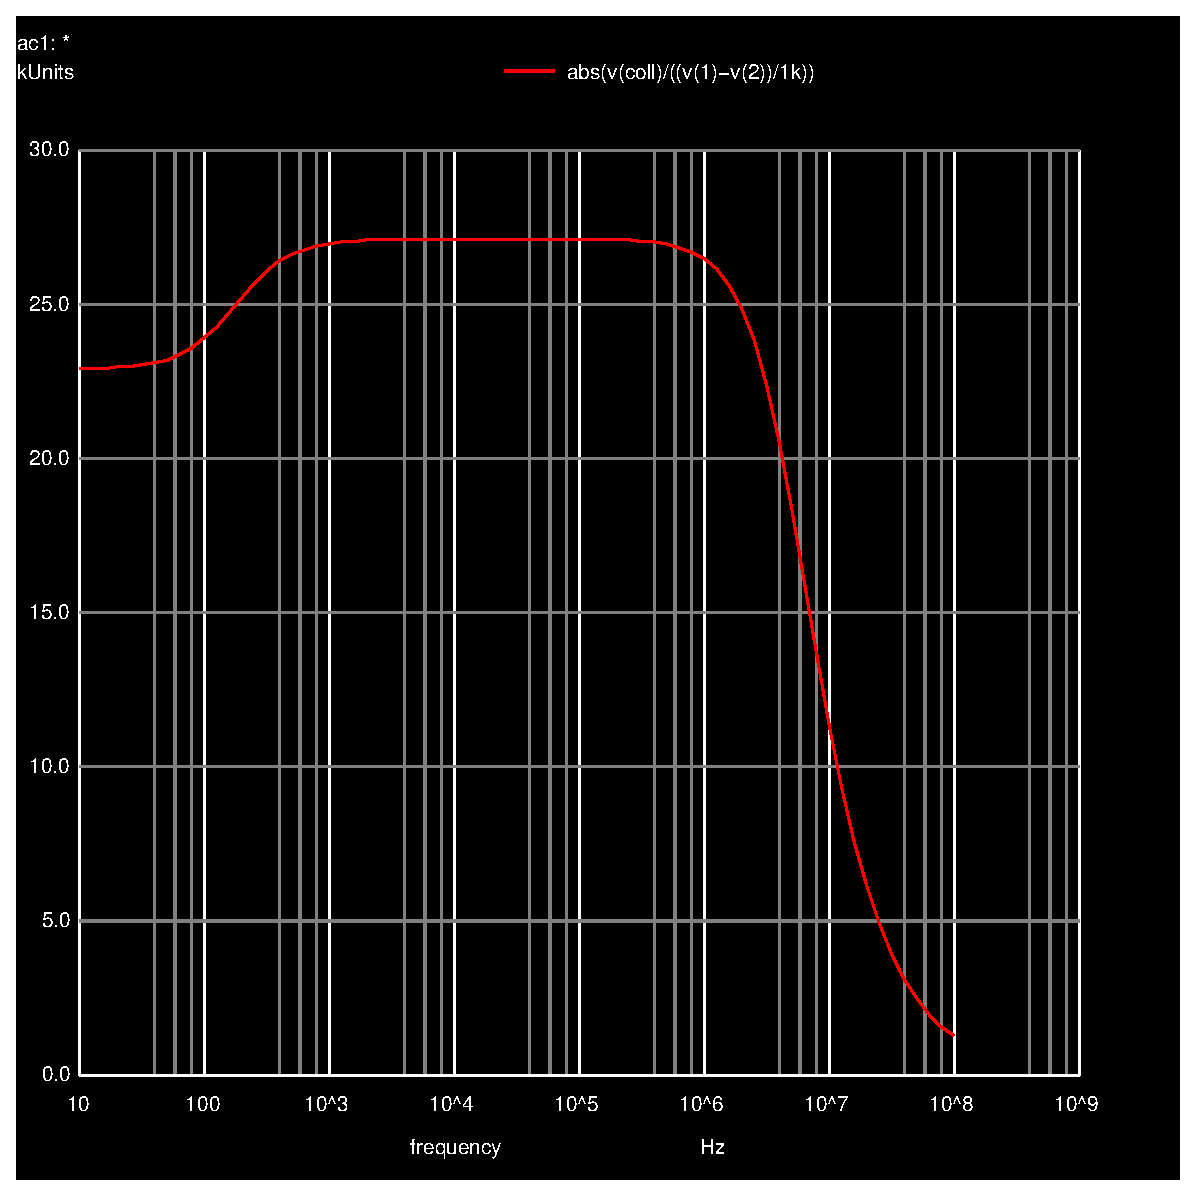
\includegraphics[width=0.6\linewidth]{zim.eps}
\caption{Input impedance}
\label{fig:zim}
\end{figure}

\lipsum[1-1]



